\documentclass[12pt,a4paper,table]{article}

\usepackage[a4paper,
            tmargin=2cm,
            bmargin=2cm,
            lmargin=2cm,
            rmargin=2cm,
            bindingoffset=0cm]{geometry}

\usepackage{lmodern}
\usepackage[T1]{polski}
\usepackage[utf8]{inputenc}
\usepackage{tocloft}
\usepackage{hyperref}
\usepackage{amsmath}
\usepackage{listings}
\usepackage{graphicx}
\usepackage{subfig}
\usepackage{float}
\usepackage{booktabs}

\hypersetup{
    colorlinks,
    citecolor=black,
    filecolor=black,
    linkcolor=black,
    urlcolor=black
}

\newtheorem{definition}{Def}


\begin{document}
    \title {
        Rachunek Macierzowy i Statystyka Wielowymiarowa \\
        Sprawozdanie 1 \\
        Mnożenie macierzy

    }

    \author{
        Adam Staniszewski \\
        Przemysław Węglik
    }

    \date{\today}

    \maketitle

    \tableofcontents
    \newpage

    \section{Algorytm Tradycyjny}

    \subsection{Opis algorytmu}
    Polega na przeiterowanie przez wszystkie elementy macierzy wynikowej i obliczenia dla nich iloczynów skalarnych odopwiadających kolumn i wierszy.
    Matematycznie możemy to zapisać jako:
    $$
    c_{ij}
    =
    \sum_{k=1}^{m} a_{ik}b_{kj} \\
    $$
    gdzie $a_{ik}$  i $b_{kj}$ to elementy macierzy, których mnożenia dokonujemy, a $c_{ij}$ to elementy macierzy wynikowej
    
    \subsection{Kod algorytmu}
    \begin{lstlisting}[language=Python]
    def traditional_method(A: np.ndarray, B: np.ndarray, counter: Counter):
        add = counter.add
        mul = counter.mul
        
        rows_A, cols_A = A.shape
        rows_B, cols_B = B.shape
        
        result = np.zeros((rows_A, cols_B))

        for i in range(rows_A):
            for j in range(cols_B):
                for k in range(cols_A):
                    result[i][j] = add(result[i][j], mul(A[i][k], B[k][j]))
        
        return result
    \end{lstlisting}

    \subsection{Benchmarki}

    \begin{figure}[H]
        \centering
        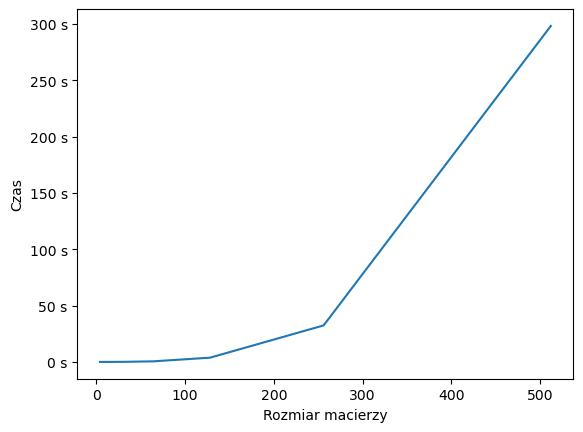
\includegraphics[width=0.6\linewidth]{img/trad_times.png}
        \caption{Wykres czasu od rozmiaru macierzy}
        \label{fig:binet_times}
    \end{figure}

    \begin{figure}[H]
        \centering
        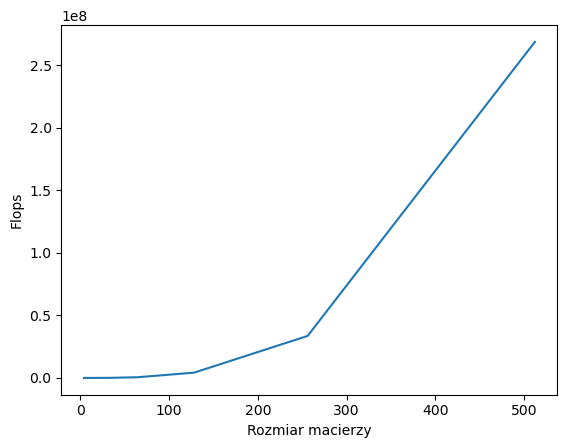
\includegraphics[width=0.6\linewidth]{img/trad_flops.png}
        \caption{Wykres ilości operacji od rozmiaru macierzy}
        \label{fig:binet_flops}
    \end{figure}

    \subsection{Analiza złożoności}
    W każdym mnożeniu macierzy o rozmiarze $n$ dokonujemy trzykrotnie zagnieżdżonej iteracji o długości równej rozmiarze macierzy.
    To prowadzi nas do złożoności $O(n^{3})$

    \newpage

    \section{Algorytm Binét'a}

    \subsection{Opis algorytmu}
    Polega na rekurencyjnym rozbijaniu macierzy na 4 mniejsze i 
    obliczaniu wyników dla tych podproblemów. Tam ponownie
    będziemy musieli użyć mnożenia i wykorzystamy procedurę.
    To klasyczne podejście nosi nazwę "divide and conquer".
    Stosujemy wzór:
    $$
    \begin{bmatrix}
        A_{11} & A_{12} \\
        A_{21} & A_{22} \\ 
    \end{bmatrix}
    \times
    \begin{bmatrix}
        B_{11} & B_{12} \\
        B_{21} & B_{22} \\ 

    \end{bmatrix}
    =
    \begin{bmatrix}
        (A_{11}B_{11} + A_{12}B_{21}) & (A_{11}B_{21} + A_{12}B_{22}) \\
        (A_{21}B_{11} + A_{22}B_{21}) & (A_{21}B_{12} + A_{22}B_{22}) \\ 
    \end{bmatrix}
    $$
    
    \subsection{Kod algorytmu}
    \begin{lstlisting}[language=Python]
        def binet_core_algorithm(A: np.ndarray, B: np.ndarray, counter: Counter) -> np.ndarray:
        add = counter.add
        mul = counter.mul
        
        if A.size > 1:
            split_at = A.shape[0] // 2
            A11, A12, A21, A22 = split(A, split_at, split_at)
            B11, B12, B21, B22 = split(B, split_at, split_at)

            C11 = add(
                binet_core_algorithm(A11, B11, counter),
                binet_core_algorithm(A12, B21, counter),
            )
            C12 = add(
                binet_core_algorithm(A11, B12, counter),
                binet_core_algorithm(A12, B22, counter),
            )     
            C21 = add(
                binet_core_algorithm(A21, B11, counter),
                binet_core_algorithm(A22, B21, counter),
            )
            
            C22 = add(
                binet_core_algorithm(A21, B12, counter),
                binet_core_algorithm(A22, B22, counter),
            )

            return np.concatenate(
                [np.concatenate([C11, C12], axis=1), np.concatenate([C21, C22], axis=1)],
                axis=0,
            )
        
        else:
            return mul(A, B)

    def binet_algorithm(A: np.ndarray, B: np.ndarray, counter: Counter) -> np.ndarray:
        new_A, new_B = resize_matrix_to_2n(A, B)
        C = binet_core_algorithm(new_A, new_B, counter)
        C = C[~np.all(C == 0, axis=1)]
        C = C[:, ~np.all(C == 0, axis=0)]
        return C
    
    \end{lstlisting}

    \subsection{Benchmarki}

    \begin{figure}[H]
        \centering
        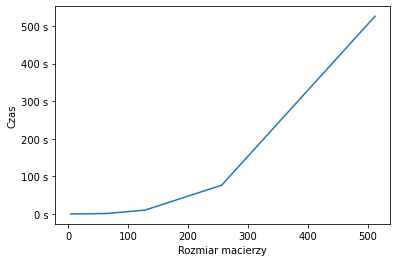
\includegraphics[width=0.6\linewidth]{img/binet_times.png}
        \caption{Wykres czasu od rozmiaru macierzy}
        \label{fig:binet_times}
    \end{figure}

    \begin{figure}[H]
        \centering
        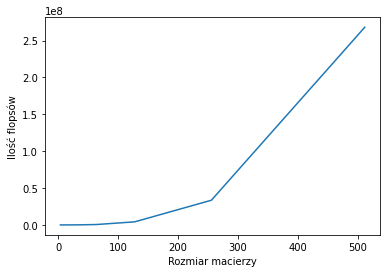
\includegraphics[width=0.6\linewidth]{img/binet_flops.png}
        \caption{Wykres ilości operacji od rozmiaru macierzy}
        \label{fig:binet_flops}
    \end{figure}

    \subsection{Analiza złożoności}
    W każdym mnożeniu macierzy o rozmiarze $n$ wykonujemy 8 podwywołań
    algorytmu na macierzach o rozmiarzach $n/2$. Taka rekurencja prowadzi do
    złożoności $O(n^{log_2(8)}) = O(n^{3})$  (twierdzenie o rekurencji uniwersalnej).

    \newpage


\end{document}